%%%%%%%%%%%%%%%%%%%%%%%%%%%%%%%%%%%%%%%%%

%%%%%%%%%%%%%%%%%%%%%%%%%%%%%%%%%%%%%%%%%

%----------------------------------------------------------------------------------------
%	PACKAGES AND DOCUMENT CONFIGURATIONS
%----------------------------------------------------------------------------------------

\documentclass[https://www.overleaf.com/project/63761df255a8a9f4a15c3579
	letterpaper, % Paper size, specify a4paper (A4) or letterpaper (US letter)
	10pt, % Default font size, specify 10pt, 11pt or 12pt
]{CSUniSchoolLabReport}


\usepackage{hyperref}
\usepackage[normalem]{ulem}
\usepackage{listings}
\usepackage{xcolor}
\definecolor{codegreen}{rgb}{0,0.6,0}
\definecolor{codegray}{rgb}{0.5,0.5,0.5}
\definecolor{codepurple}{rgb}{0.58,0,0.82}
\definecolor{backcolour}{rgb}{1,1,1}
\lstdefinestyle{mystyle}{
    backgroundcolor=\color{backcolour},   
    commentstyle=\color{codegreen},
    keywordstyle=\color{magenta},
    numberstyle=\tiny\color{codegray},
    stringstyle=\color{codepurple},
    basicstyle=\ttfamily\footnotesize,
    breakatwhitespace=false,         
    breaklines=true,                 
    captionpos=b,                    
    keepspaces=true,                 
    numbers=left,                    
    numbersep=5pt,                  
    showspaces=false,                
    showstringspaces=false,
    showtabs=false,                  
    tabsize=2
}

\lstset{style=mystyle}
\renewcommand\ULthickness{1.0pt}   %%---> For changing thickness of underline
\setlength\ULdepth{1.3ex}%\maxdimen ---> For changing depth of underline

%----------------------------------------------------------------------------------------
%	REPORT INFORMATION
%----------------------------------------------------------------------------------------


\begin{document}

\begin{figure}[H] % [H] forces the figure to be placed exactly where it appears in the text
	\centering % Horizontally center the figure
	
\includegraphics[width=0.4\textwidth]{images/logo.png} % Include the figure
\end{figure}

\begin{center}
    \begin{tabular} {c}
        \Huge Universidad La Salle \\\\\\\\
        \huge Fundamentos de Lenguajes de Programación \\\\\\\\
        \LARGE Informe de la Práctica 17 \\\\\\\\
        \huge Manipulación de Imágenes y Paralelismo en Go \\\\\\\\
        \LARGE Karlo Emigdio Pacha Curimayhua \\\\\\\\
        \LARGE Quinto Semestre - Ingeniería de Software \\\\\\\\
        \LARGE 2022
      \end{tabular}
\end{center}

\begin{center}
	\begin{tabular}{l r}
	\end{tabular}
\end{center}

%----------------------------------------------------------------------------------------
%	Ejercicio 1
%----------------------------------------------------------------------------------------

\section*{Ejercicio 1 }

\subsection*{Enunciado}
Implemente la adición de imágenes con los elementos de la Figura 1. Considere el problema de overflow en los pixeles, esto sucede cuando un pixel supera el valor de 255 o es inferior a 0; por ejemplo si un pixel resulta con un valor mayor a 255, solo le asigna el valor de 255.

\begin{figure}[H]
    \centering 
    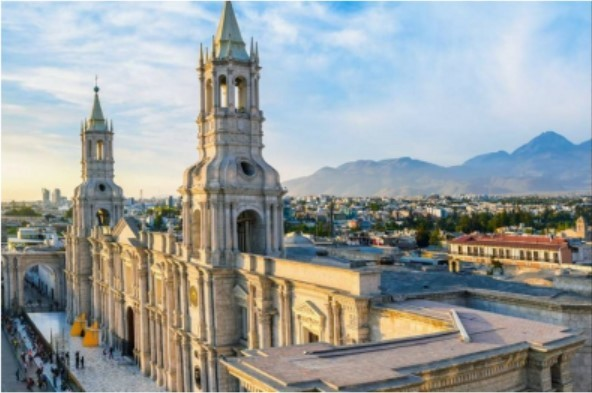
\includegraphics[width=.4\textwidth]{images/5.jpg}
    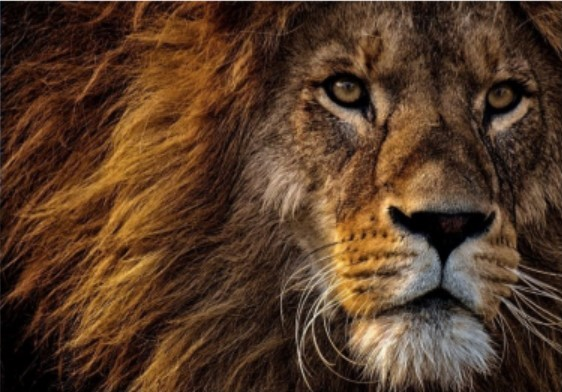
\includegraphics[width=.38\textwidth]{images/6.jpg}
    \caption{Imágenes de muestra.}
    \label{fig}
\end{figure}
%%%%%%%%%%%%%%%%%%%%%%%%%%%%%%%%%%%%%%%%
\subsection*{Solución Secuencial}

\lstinputlisting[language=go]{codes/1.1.go}

\begin{figure}[H]
    \centering 
    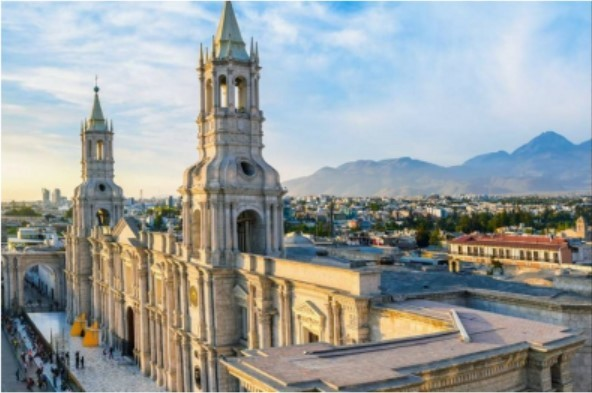
\includegraphics[width=.315\textwidth]{images/5.jpg}
    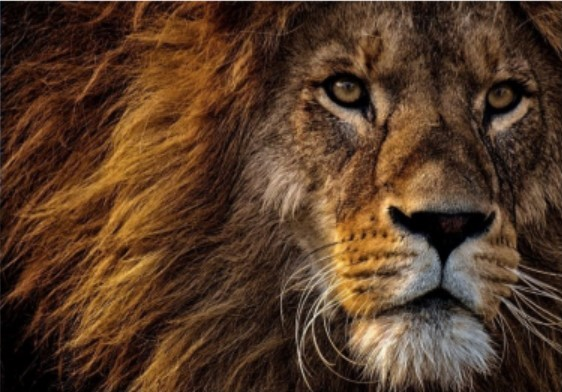
\includegraphics[width=.3\textwidth]{images/6.jpg}
    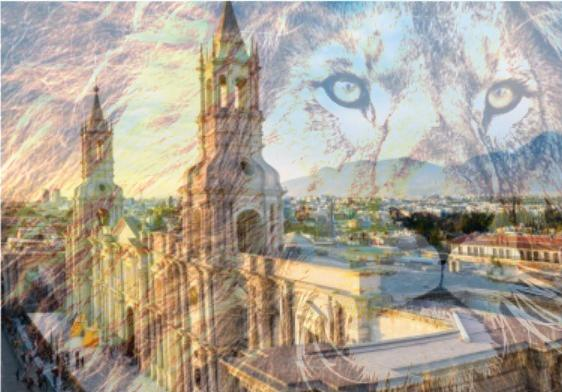
\includegraphics[width=.3\textwidth]{images/resultSequential1.jpg}
    \caption{Imágenes de entrada y resultado.}
    \label{fig}
\end{figure}
%%%%%%%%%%%%%%%%%%%%%%%%%%%%%%%%%%%%%%%%
\subsection*{Solución Paralela}

\lstinputlisting[language=go]{codes/1.2.go}

\begin{figure}[H]
    \centering 
    
\includegraphics[width=.3\textwidth]{images/1.jpg}
    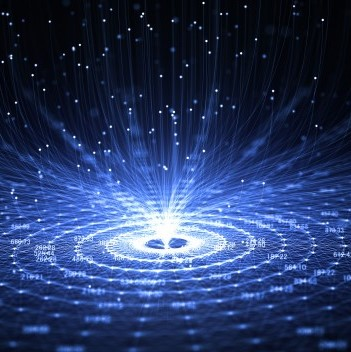
\includegraphics[width=.3\textwidth]{images/2.jpg}
    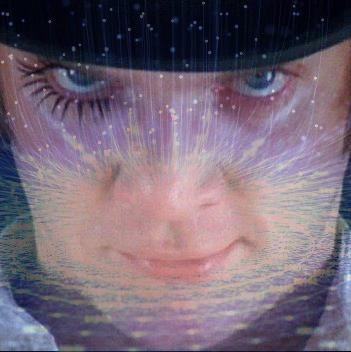
\includegraphics[width=.3\textwidth]{images/resultParallel1.jpg}
    \caption{Imágenes de entrada y resultado.}
    \label{fig}
\end{figure}
%%%%%%%%%%%%%%%%%%%%%%%%%%%%%%%%%%%%%%%%
\subsection*{Análisis}
\begin{center}
    \begin{tabular}{| c | c |}
        \hline
            Implementación & Tiempo 
             \\ 
        \hline
            Secuencial & 36.6312ms
            \\
            Paralelo & 12.9794ms
            \\
        \hline
    \end{tabular}
\end{center}
 \begin{center}
    Table 1 : Tiempos de ejecución
 \end{center}

La unión de imágenes no presenta difucultad alguna, la imagen que hará de máscara se necesita quemar. Esto se logra con la manipulación de los valores RGBA, aunque sólo basta los 3 primeros valores.
\\
A pesar de varias pruebas, la implementación paralela es 3 veces mejor que la secuencial, se saca mayor provecho de los threads en los bucles, aunque sólo se debe limitar a un número pequeño (en este caso 7) dado la enorme tamaño de las imágenes. 

%----------------------------------------------------------------------------------------
%	Ejercicio 2
%----------------------------------------------------------------------------------------

\section*{Ejercicio 2 }

\subsection*{Enunciado}
El operador blending, es un operador que suma dos imágenes, pero nosotros podemos decidir que imágen tendrá más presencia en el resultado. Implemente el operador Blending (ecuación 1) y evalue sus resultados con imágenes de su preferencia, tambien pruebe diferentes valores de x.
\\
\begin{center}
    \(Q(i,j)=X*P_{1}(i,j)+(1-X)*P_{2}(i,j)\) \ \ (1)
\end{center}
\\
Donde: \(Q(i, j)\), es un pixel de la imagen resultado; \(P_{1}(i, j)\), es un pixel de la imagen de entrada; \(P_{2}(i, j)\), es un pixel de la otra imagen de entrada.
//
Por ejemplo, con las imágenes de entrada de la Figura 4, se puede obtener el resultado de la
Figura 5, para un \(x = 0,25, x = 0,5 y x = 0,75\).

\begin{figure}[H]
    \centering 
    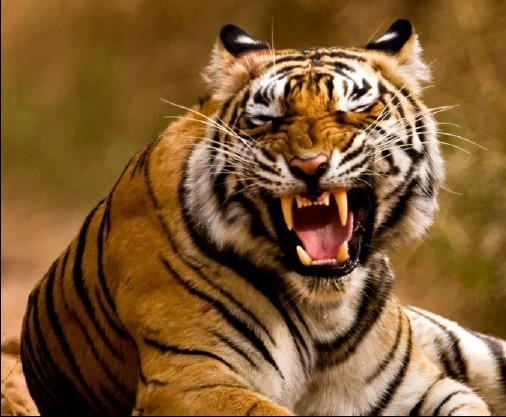
\includegraphics[width=.4\textwidth]{images/9.jpg}
    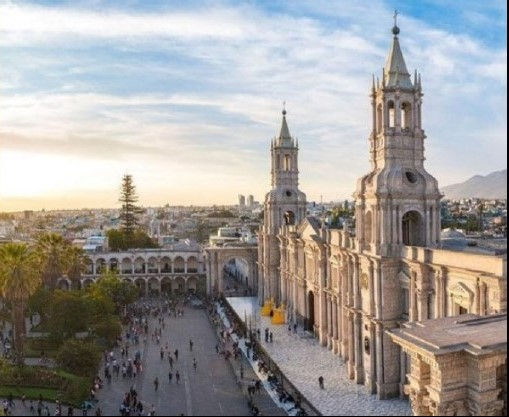
\includegraphics[width=.4\textwidth]{images/10.jpg}
    \caption{Imágenes de entrada.}
    \label{fig}
\end{figure}

\begin{figure}[H]
    \centering 
    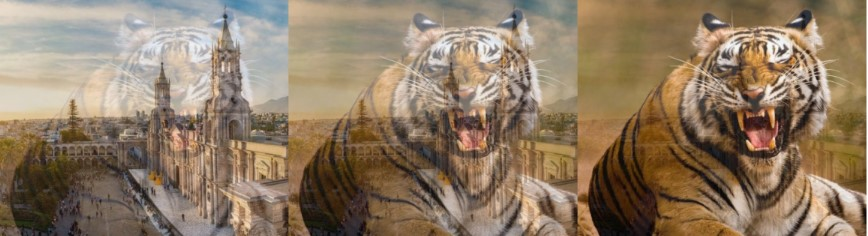
\includegraphics[width=1\textwidth]{images/12.jpg}
    \caption{Imagen resultado de blending, para \(x = 0,25, x = 0,5 y x = 0,75\).}
    \label{fig}
\end{figure}
%%%%%%%%%%%%%%%%%%%%%%%%%%%%%%%%%%%%%%%%
\subsection*{Solución Secuencial}

\lstinputlisting[language=go]{codes/2.1.go}

\begin{figure}[H]
    \centering 
    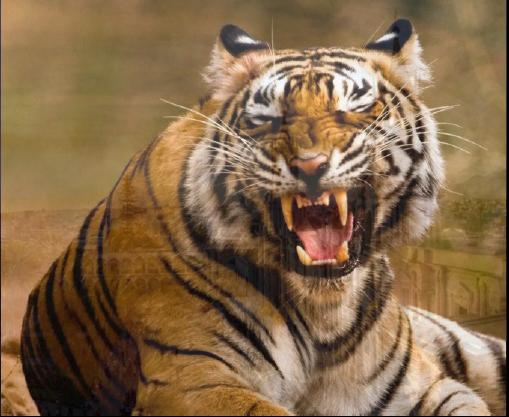
\includegraphics[width=.3\textwidth]{images/resultSequential2_25.jpg}
    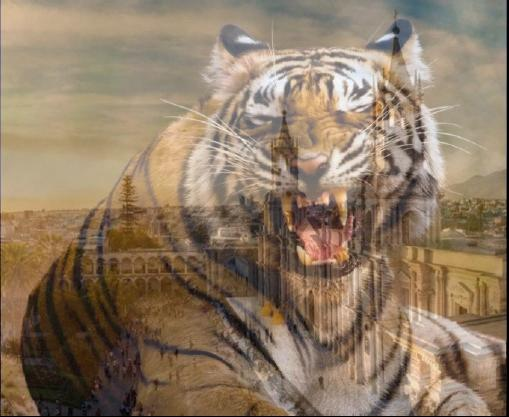
\includegraphics[width=.3\textwidth]{images/resultSequential2_50.jpg}
    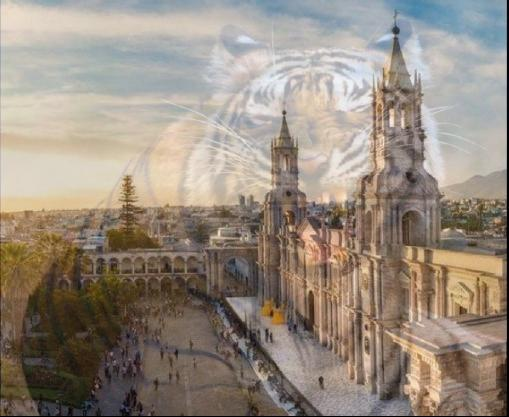
\includegraphics[width=.3\textwidth]{images/resultSequential2_75.jpg}
    \caption{Resultados.}
    \label{fig}
\end{figure}

%%%%%%%%%%%%%%%%%%%%%%%%%%%%%%%%%%%%%%%%
\subsection*{Solución Paralela}

\lstinputlisting[language=go]{codes/2.2.go}

\begin{figure}[H]
    \centering 
    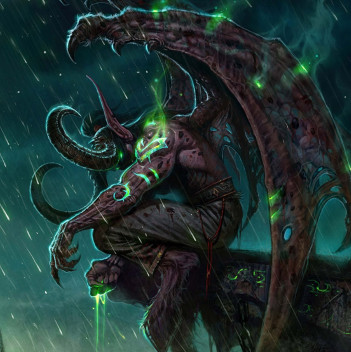
\includegraphics[width=.3\textwidth]{images/3.jpg}
    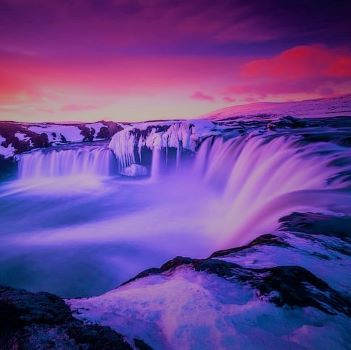
\includegraphics[width=.3\textwidth]{images/4.jpg}
    \caption{Imágenes de entrada.}
    \label{fig}
\end{figure}

\begin{figure}[H]
    \centering 
    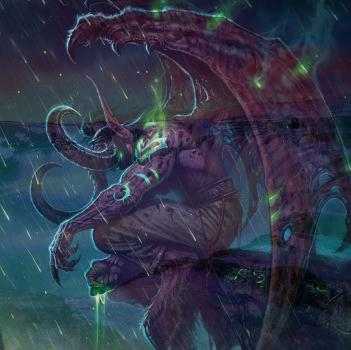
\includegraphics[width=.3\textwidth]{images/resultParallel2_25.jpg}
    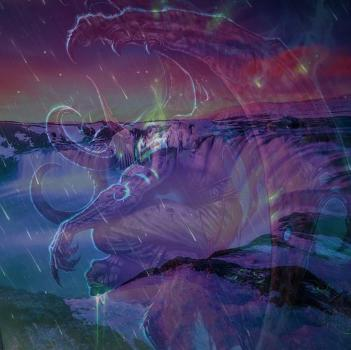
\includegraphics[width=.3\textwidth]{images/resultParallel2_50.jpg}
    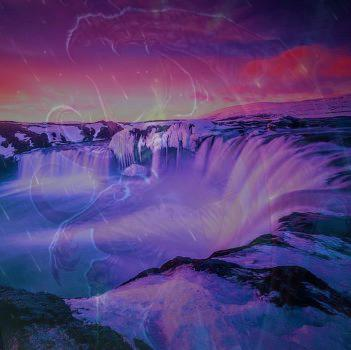
\includegraphics[width=.3\textwidth]{images/resultParallel2_75.jpg}
    \caption{Resultados.}
    \label{fig}
\end{figure}
%%%%%%%%%%%%%%%%%%%%%%%%%%%%%%%%%%%%%%%%
\subsection*{Análisis}
\begin{center}
    \begin{tabular}{| c | c |}
        \hline
            Implementación & Tiempo 
             \\ 
        \hline
            Secuencial & 45.6795ms
            \\
            Paralelo & 18.5831ms
            \\
        \hline
    \end{tabular}
\end{center}
 \begin{center}
    Table 2 : Tiempos de ejecución
 \end{center}

A la imagen de máscara se le necesita manipular los valores Alpha, en este caso a menor valor tenga \(X\), mayor transparencia.
\\
A pesar de varias pruebas, nuevamente la implementación paralela es 2.5 veces mejor que la secuencial, se saca mayor provecho de los threads en los bucles, aunque sólo se debe limitar a un número pequeño (en este caso 3 y 2) dado la enorme tamaño de las imágenes y los 3 niveles de transparencia. 
%----------------------------------------------------------------------------------------
%	Ejercicio 3
%----------------------------------------------------------------------------------------

\section*{Ejercicio  3 }

\subsection*{Enunciado}
Obtenga el histograma de una imagen, este representa la frecuencia de intensidad de un colores de los pixeles.Como un pixel tiene tres canales de colores, se puede obtener tres histogramas como se ve en la Figura 9.

\begin{figure}[H]
    \centering 
    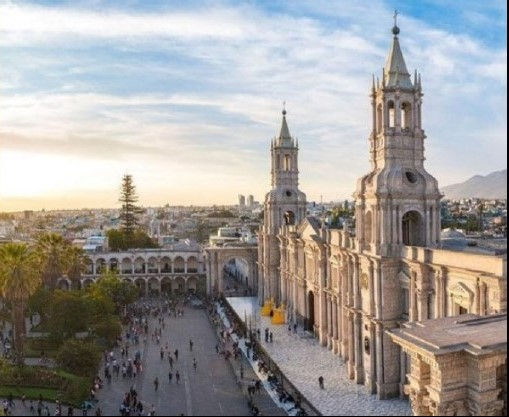
\includegraphics[width=.4\textwidth]{images/10.jpg}
    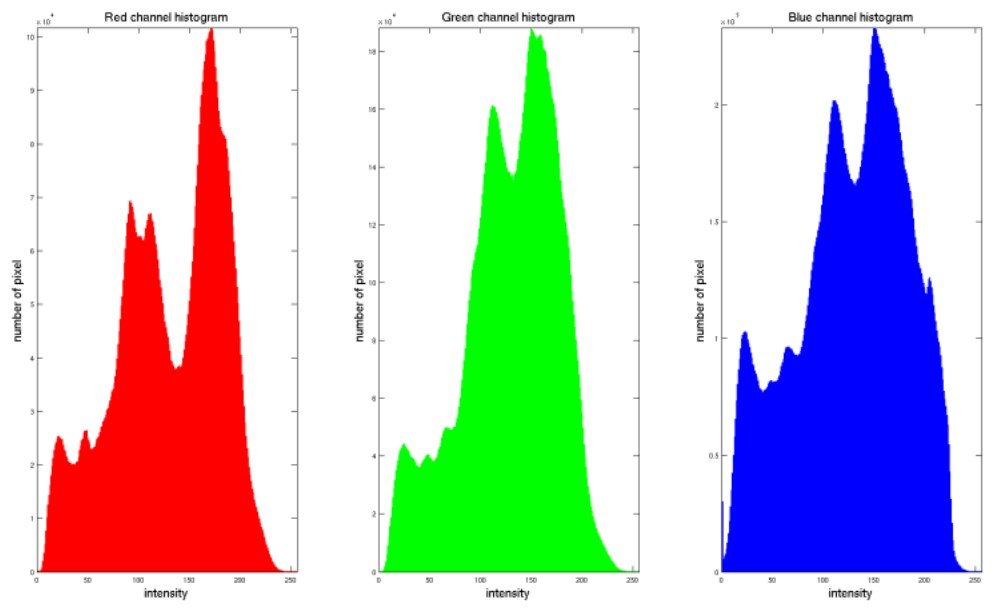
\includegraphics[width=.55\textwidth]{images/13.jpg}
    \caption{Ejemplo de histograma de una imagen.}
    \label{fig}
\end{figure}
%%%%%%%%%%%%%%%%%%%%%%%%%%%%%%%%%%%%%%%%
\subsection*{Solución Secuencial}

\lstinputlisting[language=go]{codes/3.1.go}

\begin{figure}[H]
    \centering 
    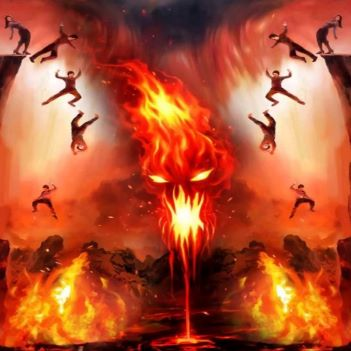
\includegraphics[width=.315\textwidth]{images/8.jpg}
    \caption{Imagen de entrada.}
    \label{fig}
\end{figure}

\begin{figure}[H]
    \centering 
    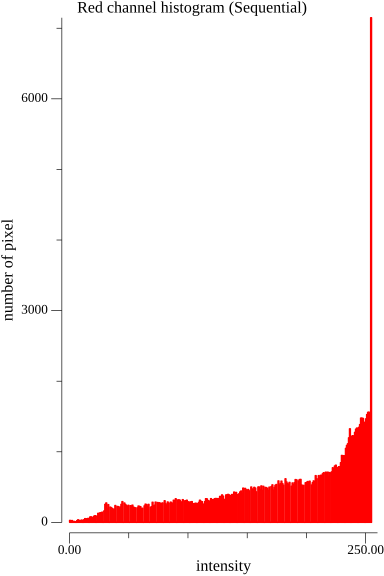
\includegraphics[width=.315\textwidth]{images/redHistogramSequential.png}
    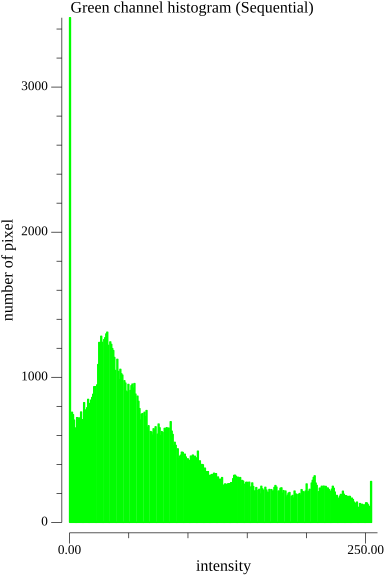
\includegraphics[width=.3\textwidth]{images/greenHistogramSequential.png}
    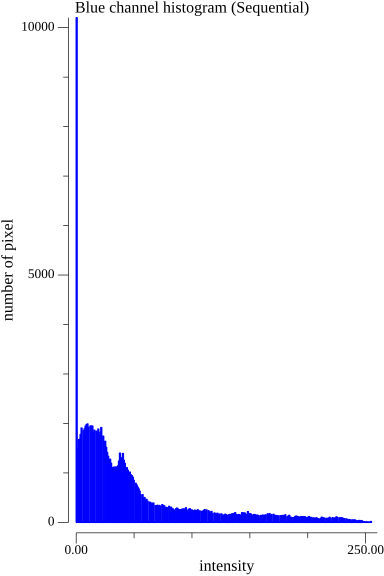
\includegraphics[width=.3\textwidth]{images/blueHistogramSequential.png}
    \caption{Histogramas resultantes.}
    \label{fig}
\end{figure}
%%%%%%%%%%%%%%%%%%%%%%%%%%%%%%%%%%%%%%%%
\subsection*{Solución Paralela}

\lstinputlisting[language=go]{codes/1.2.go}

\begin{figure}[H]
    \centering 
    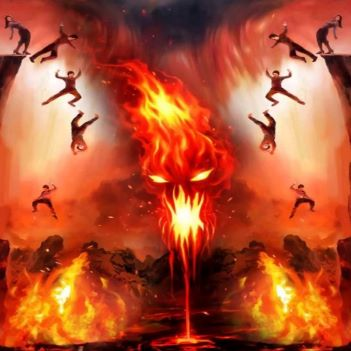
\includegraphics[width=.315\textwidth]{images/8.jpg}
    \caption{Imagen de entrada.}
    \label{fig}
\end{figure}

\begin{figure}[H]
    \centering 
    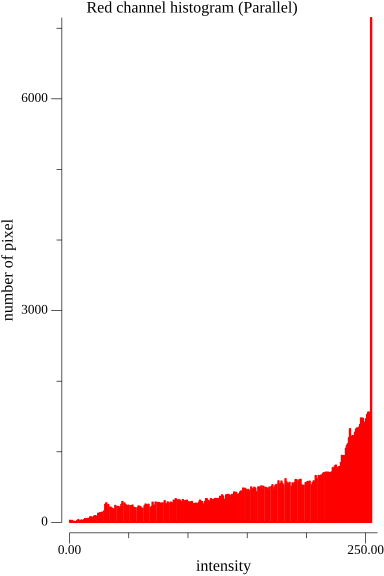
\includegraphics[width=.3\textwidth]{images/redHistogramParallel.png}
    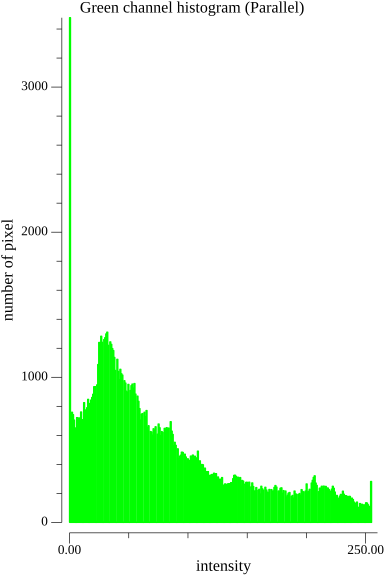
\includegraphics[width=.3\textwidth]{images/greenHistogramParallel.png}
    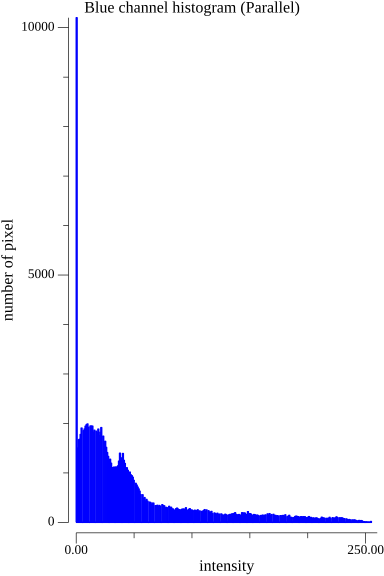
\includegraphics[width=.3\textwidth]{images/blueHistogramParallel.png}
    \caption{Imágenes de entrada y resultado.}
    \label{fig}
\end{figure}
%%%%%%%%%%%%%%%%%%%%%%%%%%%%%%%%%%%%%%%%
\subsection*{Análisis}
\begin{center}
    \begin{tabular}{| c | c |}
        \hline
            Implementación & Tiempo 
             \\ 
        \hline
            Secuencial & 68.0478ms
            \\
            Paralelo & 50.7469ms
            \\
        \hline
    \end{tabular}
\end{center}
 \begin{center}
    Table 3 : Tiempos de ejecución
 \end{center}

Para la obtención de los valores RGB se usa la misma lógica. Para graficar los histogramas se necesita el módulo 
\boldsymbol{"gonum.org/v1/plot"}, este también usa otros como : \boldsymbol{"gonum.org/v1/plot/plotter"} y \boldsymbol{"gonum.org/v1/plot/vg"}. Se debe crear un función especial (Histogram).
\\
A pesar de varias pruebas, la implementación paralela es mejor que la secuencial, aunque esta vez no por tanto. En este caso no se puedo sacar mucho provecho a los threads dado errores al exportar o generar los histogramas, sólo se pudo usar uno para obtener uno de los histogramas.

%----------------------------------------------------------------------------------------
%	Ejercicio 3
%----------------------------------------------------------------------------------------

\section*{Conclusión}
Go demostró ser tan bueno como python para manipular imágenes y generar gráficos, aunque quizás no tiene tanta facilidad como python. Para el manejo de threads se muestra simple aunque si se debe prestar atención a como se programa estos.
\\
%----------------------------------------------------------------------------------------
\\
\href{https://github.com/KEPCU/FundamentalsOfProgrammingLanguages/tree/master/go/practice17}{GitHub} : \url{https://github.com/KEPCU/FundamentalsOfProgrammingLanguages/tree/master/go/practice17}

%----------------------------------------------------------------------------------------

\end{document}